\documentclass[pdflatex,sn-mathphys-num]{sn-jnl}% Math and Physical Sciences Numbered


\usepackage{graphicx}%
\usepackage{multirow}%
\usepackage{amsmath,amssymb,amsfonts}%
\usepackage{amsthm}%
\usepackage{mathrsfs}%
\usepackage[title]{appendix}%
\usepackage{xcolor}%
\usepackage{textcomp}%
\usepackage{manyfoot}%
\usepackage{booktabs}%
\usepackage{algorithm}
\usepackage{algorithmicx}
\usepackage{algpseudocode}
\usepackage{multicol}
\usepackage{fancyvrb}
\usepackage{geometry}
\usepackage{titlesec}
\usepackage{xcolor}
\usepackage{parskip}

%\usepackage[backend=biber,style=apa]{biblatex} % or use another style
%\addbibresource{references.bib} % your .bib file
\usepackage{hyperref}
\usepackage{fontawesome5} % For the GitHub icon
\usepackage[justification=centering]{caption}
\usepackage[linesnumbered,ruled,vlined]{algorithm2e}
\setlength{\topmargin}{-0.4in}
\setlength{\textheight}{9in}
\usepackage{comment}
\usepackage{listings}%
% In your preamble:
\usepackage{enumitem} % For custom list formatting
\newlist{questions}{enumerate}{1}
\setlist[questions,1]{
  label=\textbf{Q\arabic*:}, % Label format "Q1:", "Q2:", ...
  leftmargin=2em,           % Indent spacing
  itemsep=1em               % Space between questions
}



%%%%


%% as per the requirement new theorem styles can be included as shown below
\theoremstyle{thmstyleone}%
\newtheorem{theorem}{Theorem}%  meant for continuous numbers
%%\newtheorem{theorem}{Theorem}[section]% meant for sectionwise numbers
%% optional argument [theorem] produces theorem numbering sequence instead of independent numbers for Proposition
\newtheorem{proposition}[theorem]{Proposition}%
%%\newtheorem{proposition}{Proposition}% to get separate numbers for theorem and proposition etc.

\theoremstyle{thmstyletwo}%
\newtheorem{example}{Example}%
\newtheorem{remark}{Remark}%

\theoremstyle{thmstylethree}%
\newtheorem{definition}{Definition}%

\raggedbottom



% Code Packages

\usepackage{listings}
\usepackage{xcolor}

\definecolor{headerbackground}{rgb}{1, 1, 1}
\definecolor{rulecolor}{rgb}{0.7, 0.7, 0.7}

% Define C keywords including standard library functions
\lstdefinestyle{algorithmstyle}{
  backgroundcolor=\color{white},
  basicstyle=\ttfamily\scriptsize,
  keywordstyle=\bfseries, % Bold for keywords
  commentstyle=\itshape, % Italic for comments
  stringstyle=,
  numberstyle=\tiny,
  numbers=left,
  numbersep=10pt,
  breaklines=true,
  frame=trbl,
  framerule=0.8pt,
  rulecolor=\color{rulecolor},
  framesep=5pt,
  xleftmargin=15pt,
  xrightmargin=5pt,
  language=C, % This is crucial
  tabsize=2,
  showstringspaces=false,
  alsoletter={\_},
  morekeywords={printf, scanf, malloc, free, sizeof, puts, gets}, % Add standard library functions
}

\newcommand{\codeheader}[1]{%
  \noindent%
  \fcolorbox{rulecolor}{headerbackground}{%
    \makebox[\dimexpr\linewidth-2\fboxsep-2\fboxrule][l]{%
      \textbf{Code:} \ttfamily{#1}%
    }%
  }%
  \vspace{-0.5\baselineskip}
}


\ExplSyntaxOn

\NewDocumentCommand{\sortedkeywords}{m}
 {
  \clist_set:Nn \l_tmpa_clist {#1}
  \seq_set_from_clist:NN \l_tmpa_seq \l_tmpa_clist
  \seq_sort:Nn \l_tmpa_seq
   {
    \str_compare:nNnTF {##1} > {##2}
     { \sort_return_swapped: }
     { \sort_return_same: }
   }
  \keywords{\seq_use:Nn \l_tmpa_seq {,~}}
 }

\ExplSyntaxOff % Necessary line to avoid errors with the next line of code (begin document)

\usepackage{xcolor}
\newcommand{\pendiente}[1]{\textcolor{red}{\textit{[PENDIENTE: #1]}}}

\begin{document}

\title[Article Title]{Proyecto Intermedio - Diseño e Implementación de un Controlador PID Analógico para una Planta RLC de Tercer Orden}

\author[1]{\fnm{Contreras R.} \sur{Orlando}}
\author[1]{\fnm{García B.} \sur{Iker}}
\author[1]{\fnm{Lara H.} \sur{Kevin}}

\affil[1]{\orgdiv{Departamento de Sistemas Electrónicos},
\orgname{Universidad Autónoma de Aguascalientes},
\orgaddress{\street{Av. Universidad 940}, \city{Aguascalientes}, \postcode{20131}, \state{Aguascalientes}, \country{México}}}

\email{\{al348390, al307630, al464376\}@edu.uaa.mx}


%%==================================%%
%% Sample for unstructured abstract %%
%%==================================%%

\abstract{En este proyecto se diseñó, simuló e implementó un controlador PID analógico en forma paralela, construido con amplificadores operacionales TL082, para mejorar la respuesta transitoria de una planta RLC serie subamortiguada.  La sintonía inicial se obtuvo por el método de oscilaciones sostenidas de Ziegler-Nichols, Debido a que esta sintonía genera un sobrepaso, se realizó un ajuste fino en MATLAB, con lo cual se obtuvo un sobrepaso de $7.6\,\%$, error en estado estable nulo y un tiempo de asentamiento de $714\,\mu\text{s}$, menor que los $790\,\mu\text{s}$ de lazo abierto. El diseño se trasladó a valores de resistencias y capacitores y se verificó en LTspice.}

\keywords{Control PID, Ziegler-Nichols, Oscilaciones sostenidas, Circuito RLC, Amplificador operacional, Filtro derivativo, MATLAB, LTspice.}


%%\pacs[JEL Classification]{D8, H51}

%%\pacs[MSC Classification]{35A01, 65L10, 65L12, 65L20, 65L70}

\maketitle
\section{Objetivo}\label{sec1}

Diseñar, simular, construir y evaluar un controlador PID analógico, implementado con amplificadores operacionales, que mejore la respuesta transitoria de una planta RLC subamortiguada, obteniendo la sintonía inicial mediante el método de oscilaciones sostenidas (Ziegler-Nichols en lazo cerrado) y refinándola mediante simulación en MATLAB, de manera que el sistema en lazo cerrado cumpla con las siguientes especificaciones:

\begin{itemize}
    \item Error en estado estable nulo ($e_{ss}=0$).
    \item Sobrepaso máximo $M_p\leq15\,\%$.
    \item Tiempo de asentamiento menor que el de lazo abierto.
\end{itemize}

\section{Materiales y Metodología}

\begin{itemize}
    \item Inductor de $10\,\text{mH}$
    \item Capacitores de $100\,\text{nF}$, $10\,\text{nF}$ y $1\,\text{nF}$
    \item Resistencias y Trimpots
    \item Amplificadores operacionales TL082
    \item Fuente de alimentación dual de $\pm12\,\text{V}$
    \item Generador de funciones (señal cuadrada de $0$ a $1\,\text{V}$, $100\,\text{Hz}$)
    \item Osciloscopio digital y multímetro
    \item Protoboard, cables de conexión y sondas
\end{itemize}
\begin{figure}[!h]
    \centering
    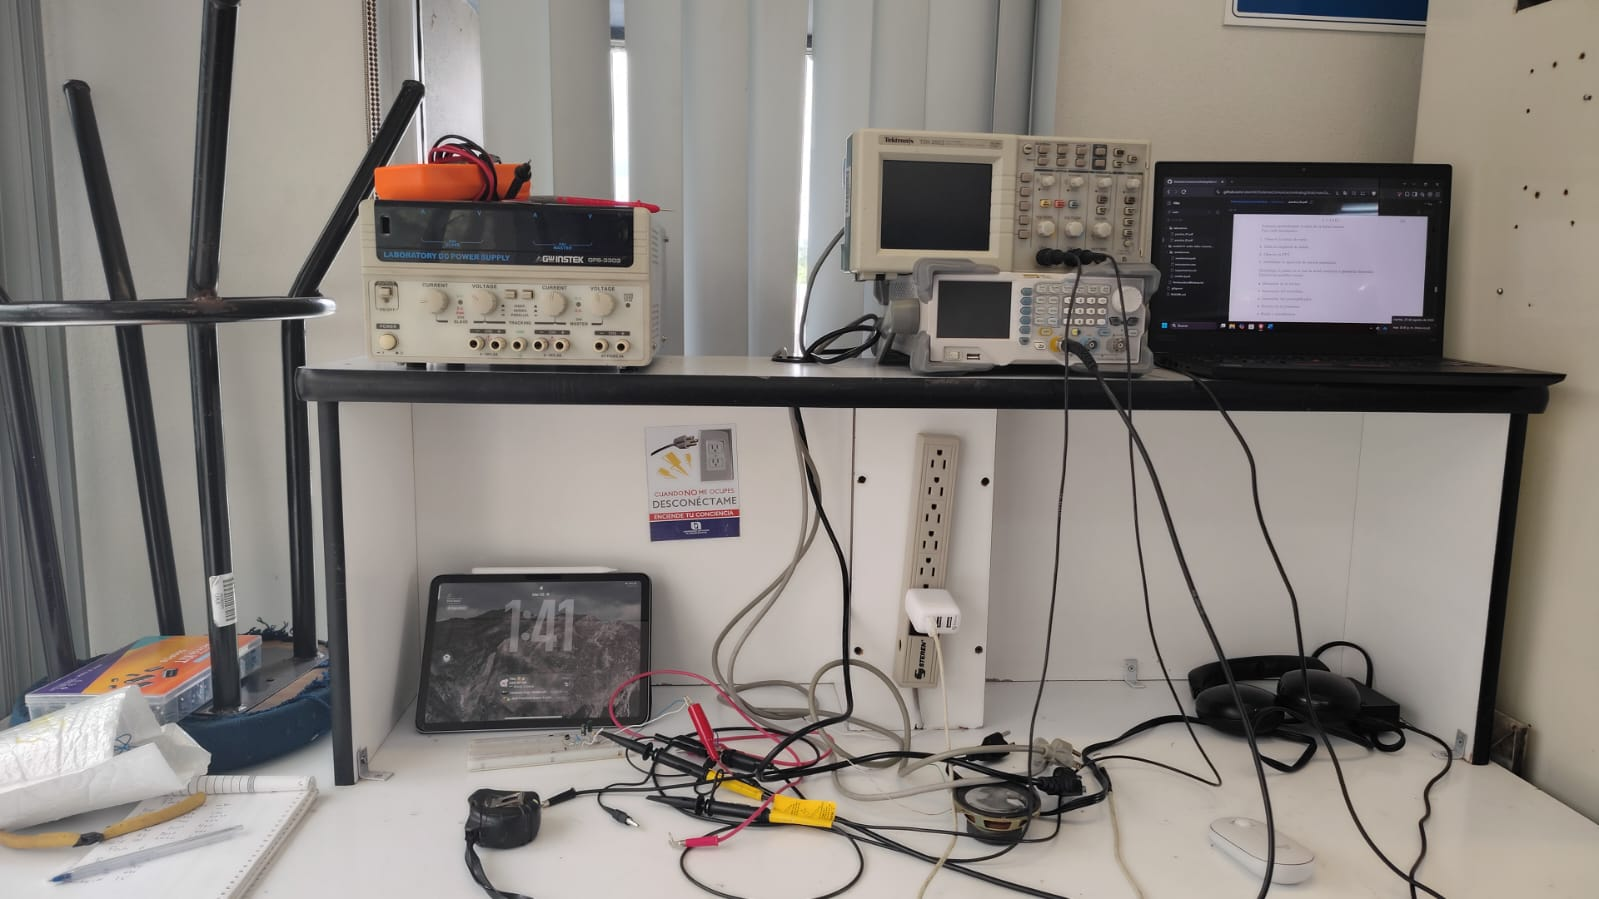
\includegraphics[width=0.7\linewidth]{src/PY_2/Triada.png}
    \caption{Materiales}
    \label{fig:placeholder}
\end{figure}

\subsection{Modelado de la Planta}

La planta se compone de un circuito RLC serie con salida en el capacitor, seguido de un seguidor de tensión, una etapa RC y un segundo seguidor de tensión. La resistencia total del lazo está formada por $R_{50}=58\,\Omega$ y $R_{35}=100\,\Omega$ en serie, más la resistencia DC del inductor (DCR) y la resistencia de salida del amplificador que excita al circuito. La función de transferencia del RLC es

\[
G_{RLC}(s)=\frac{V_C(s)}{U(s)}=\frac{\dfrac{1}{LC}}{s^2+\dfrac{R}{L}s+\dfrac{1}{LC}}=\frac{\omega_n^2}{s^2+2\zeta\omega_n s+\omega_n^2},
\]

con

\[
\omega_n=\frac{1}{\sqrt{LC}}=\frac{1}{\sqrt{(10\,\text{mH})(100\,\text{nF})}}=31\,623\,\text{rad/s}\;(5.03\,\text{kHz}),
\]
$$
\zeta=\frac{R}{2}\sqrt{\frac{C}{L}}=\frac{158.1}{2}\sqrt{\frac{100\,\text{nF}}{10\,\text{mH}}}=0.25 .$$
El valor de $\zeta$ queda dentro del intervalo requerido $0.15\leq\zeta\leq0.35$. Para este amortiguamiento, el RLC por sí solo presenta un sobrepaso teórico

\[
M_p=e^{-\zeta\pi/\sqrt{1-\zeta^2}}\times100\,\%=44.4\,\%,
\qquad
t_s\approx\frac{4}{\zeta\omega_n}=506\,\mu\text{s}.
\]

La etapa RC adicional ($R_{49}=20\,\text{k}\Omega$, $C_{14}=10\,\text{nF}$) introduce un polo real en

\[
G_{RC}(s)=\frac{1}{\tau s+1},\qquad \tau=R_{49}C_{14}=200\,\mu\text{s}\;\Rightarrow\;p_3=-5\,000\,\text{rad/s}.
\]

Los seguidores de tensión U20 y U21 aíslan las etapas, de modo que la planta completa resulta en el producto de ambas funciones:

\[
H(s)=G_{RLC}(s)\,G_{RC}(s)
=
\frac{\omega_n^2}{s^2+2\zeta\omega_n s+\omega_n^2}\frac{1}{\tau s+1}
=
\frac{5\times10^{12}}{s^3+20\,811\,s^2+1.079\times10^{9}\,s+5\times10^{12}},
\]

cuyos polos son $s_{1,2}=-7\,905\pm j30\,618\,\text{rad/s}$ y $s_3=-5\,000\,\text{rad/s}$. La ganancia en DC es $H(0)=1$.

\subsection{Sintonía Inicial: Método de Oscilaciones Sostenidas}

Con las acciones integral y derivativa desactivadas ($K_i=0$, $K_d=0$), se incrementó la ganancia proporcional hasta obtener una oscilación sostenida de amplitud constante a la salida, sin saturar los amplificadores. En el modelo, la ganancia última se obtiene con \texttt{margin(H)} como el margen de ganancia, y el periodo último a partir de la frecuencia de cruce de fase de $-180^\circ$:

\[
K_{cr}=3.49\;(10.86\,\text{dB}),\qquad \omega_{cr}=32\,848\,\text{rad/s},\qquad P_{cr}=\frac{2\pi}{\omega_{cr}}=191.3\,\mu\text{s}\;(5.23\,\text{kHz}).
\]

El mismo resultado se observa en el lugar de las raíces (Figura \ref{fig:rlocus}), donde las ramas de los polos complejos cruzan el eje imaginario en $s=\pm j32\,848\,\text{rad/s}$ para $K=3.49$.



\begin{figure}[!h]
    \centering
    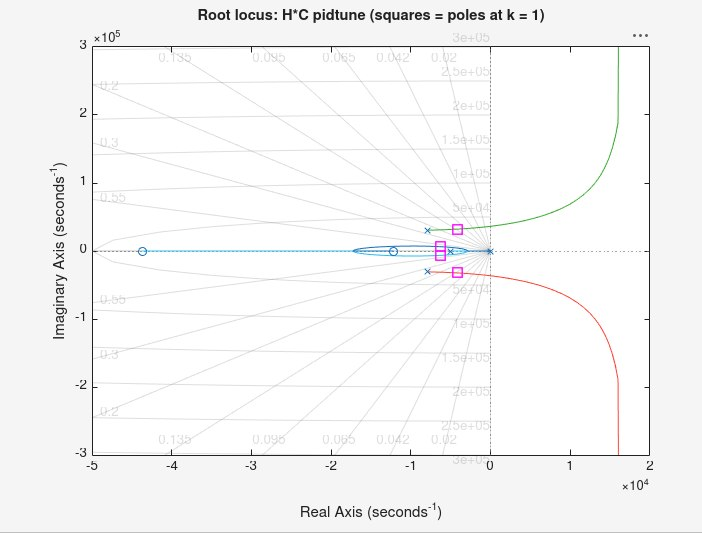
\includegraphics[width=0.7\linewidth]{src/PY_2/R_Locos.png}
    \caption{Lugar de las raíces de $H(s)$ con control proporcional.}
    \label{fig:rlocus}
\end{figure}

Aplicando la tabla de Ziegler-Nichols para un controlador PID:

\[
K_p=0.6K_{cr}=2.09,\qquad T_i=\frac{P_{cr}}{2}=95.6\,\mu\text{s},\qquad T_d=\frac{P_{cr}}{8}=23.9\,\mu\text{s},
\]

y las ganancias independientes de cada rama del circuito son

\[
K_i=\frac{K_p}{T_i}=2.19\times10^{4}\,\text{s}^{-1},\qquad K_d=K_pT_d=5.0\times10^{-5}\,\text{s}.
\]

\subsection{Simulación y Ajuste Fino en MATLAB}

El controlador se modeló en forma paralela,

\[
C(s)=K_p+\frac{K_i}{s}+K_ds,
\]

y el lazo cerrado con realimentación unitaria como $G_p(s)=\dfrac{C(s)H(s)}{1+C(s)H(s)}$. Se simuló la respuesta al escalón con \texttt{step} y se obtuvieron las métricas con \texttt{stepinfo} (criterio de asentamiento del $2\,\%$). El código completo se presenta en el Apéndice \ref{app:matlab}.

La sintonía de Ziegler-Nichols produce una respuesta rápida, pero con $M_p=18.2\,\%$, que excede la especificación de $15\,\%$. A partir de ella, el ajuste fino se realizó con el siguiente criterio:

\begin{enumerate}
    \item \textbf{Reducción de $K_p$ de $2.09$ a $1.5$:} el sobrepaso de Ziegler-Nichols proviene principalmente de la cercanía a la ganancia crítica ($K_p/K_{cr}=0.6$). Al reducir la relación a $0.43$, los polos dominantes se alejan del eje imaginario y el sobrepaso disminuye.
    \item \textbf{Reducción de $K_i$ de $2.19\times10^{4}$ a $1.2\times10^{4}\,\text{s}^{-1}$} ($T_i=125\,\mu\text{s}$): una acción integral más suave reduce la acumulación de error durante el transitorio y el sobrepaso asociado, sin perder el error en estado estable nulo.
    \item \textbf{Aumento de $K_d$ de $5.0\times10^{-5}$ a $6.7\times10^{-5}\,\text{s}$} ($T_d=44.7\,\mu\text{s}$): la acción derivativa adicional aporta fase en la zona de cruce y amortigua el modo oscilatorio del RLC.
\end{enumerate}

Con estos valores, el lazo cerrado tiene polos en $-5\,655\pm j35\,027\,\text{rad/s}$ y $-4\,751\pm j5\,009\,\text{rad/s}$, un margen de ganancia de $28.5\,\text{dB}$ y un margen de fase de $81.6^\circ$ (Figura \ref{fig:bode}).


\begin{figure}[!h]
    \centering
    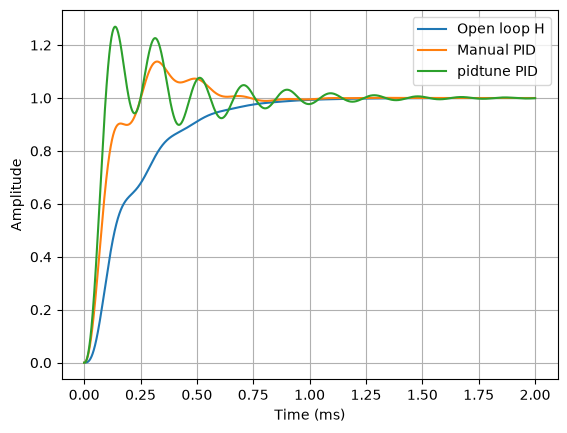
\includegraphics[width=0.7\linewidth]{src/PY_2/PID_Tune.png}
    \caption{Comparación PID manual y PID-Tune}
    \label{fig:placeholder}
\end{figure}



\begin{figure}[!h]
    \centering
    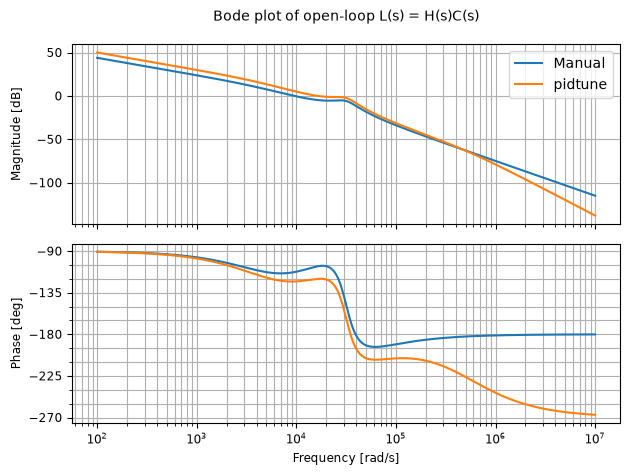
\includegraphics[width=0.7\linewidth]{src/PY_2/Bode.png}
    \caption{Diagrama de Bode de la planta $H(s)$ y del lazo abierto compensado $C(s)H(s)$.}
    \label{fig:bode}
\end{figure}



\subsection{Diseño del Circuito}

El controlador se implementó en forma paralela (Figura \ref{fig:esquematico}) con cinco etapas:

\begin{itemize}
    \item \textbf{Restador (U15):} con $R_{36}=R_{37}=R_{38}=R_{39}=10\,\text{k}\Omega$ entrega $e(t)=r(t)-y(t)$, donde $y(t)$ es la salida del seguidor U21.
    \item \textbf{Rama proporcional (U16):} amplificador inversor con ganancia $-R_{43}/R_{40}$.
    \item \textbf{Rama integral (U17):} integrador inversor con función de transferencia $-1/(R_{41}C_{12}s)$.
    \item \textbf{Rama derivativa (U18):} derivador inversor con $R_{42}$ en serie con $C_{13}$, que limita la ganancia en alta frecuencia (filtro derivativo):
    \[
    C_D(s)=-\frac{R_{44}C_{13}\,s}{R_{42}C_{13}\,s+1}.
    \]
    \item \textbf{Sumador inversor (U19):} con $R_{45}=R_{46}=R_{47}=R_{48}=10\,\text{k}\Omega$ suma las tres ramas y corrige el signo, de modo que la doble inversión entrega $u(t)$ con signo positivo.
\end{itemize}

Los valores de componentes se obtuvieron a partir de las ganancias finales (Tabla \ref{tab:componentes}).

\begin{table}[h]
\centering
\caption{Cálculo de los componentes del PID analógico.}
\label{tab:componentes}
\begin{tabular}{lccc}
\hline
\textbf{Rama} & \textbf{Relación} & \textbf{Componentes} & \textbf{Ganancia obtenida} \\
\hline
P & $K_p=R_{43}/R_{40}$ & $R_{40}=10\,\text{k}\Omega$, $R_{43}=15\,\text{k}\Omega$ & $K_p=1.5$ \\
I & $K_i=1/(R_{41}C_{12})$ & $R_{41}=83.33\,\text{k}\Omega$, $C_{12}=1\,\text{nF}$ & $K_i=1.2\times10^{4}\,\text{s}^{-1}$ \\
D & $K_d=R_{44}C_{13}$ & $R_{44}=65\,\text{k}\Omega$, $C_{13}=1\,\text{nF}$ & $K_d=6.5\times10^{-5}\,\text{s}$ \\
Filtro D & $\tau_f=R_{42}C_{13}$ & $R_{42}=2.4\,\text{k}\Omega$ & $\tau_f=2.4\,\mu\text{s}$ \\
\hline
\end{tabular}
\end{table}

$R_{41}=83.33\,\text{k}\Omega$ no es un valor comercial; se implementa con $82\,\text{k}\Omega+1.3\,\text{k}\Omega$ en serie o con un potenciómetro de $100\,\text{k}\Omega$ ajustado. Para $R_{44}$ se usó $65\,\text{k}\Omega$, lo que da $K_d=6.5\times10^{-5}\,\text{s}$, $3\,\%$ por debajo del valor de diseño; con $68\,\text{k}\Omega$ (E12) se obtendría $6.8\times10^{-5}\,\text{s}$. El polo del filtro derivativo queda en $1/\tau_f=417\,\text{krad/s}$, unas $13$ veces por encima de $\omega_n$, de modo que no afecta la dinámica de interés y sí limita la amplificación del ruido de alta frecuencia. Para el reinicio del integrador se agrega un interruptor en paralelo con $C_{12}$, que se cierra durante la búsqueda de $K_{cr}$ y antes de cada prueba al escalón.


\begin{figure}[!h]
    \centering
    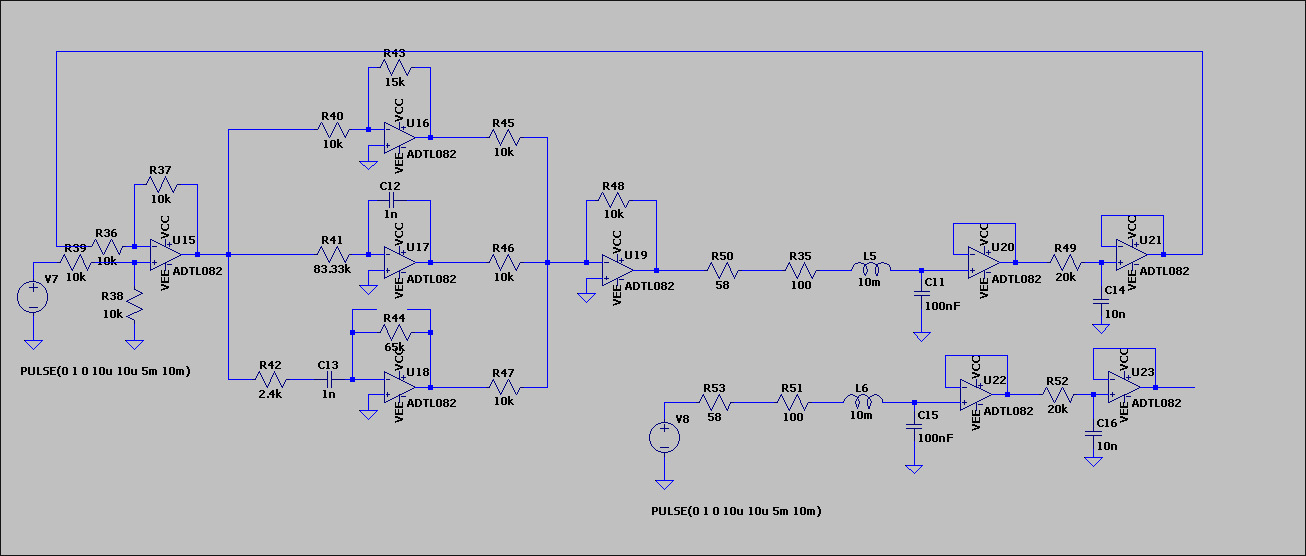
\includegraphics[width=0.8\linewidth]{src/PY_2/Schematic.png}
    \caption{Esquemático en LTspice del sistema completo: restador, ramas P, I y D, sumador, planta RLC con etapa RC en lazo cerrado (arriba) y planta en lazo abierto de referencia (abajo).}
    \label{fig:esquematico}
\end{figure}

En LTspice se simuló el sistema completo con amplificadores TL082 y una señal de referencia \texttt{PULSE(0 1 0 10u 10u 5m 10m)}. Además del lazo cerrado, se incluyó una copia de la planta excitada directamente por la misma señal (V8), para comparar las respuestas de lazo abierto y lazo cerrado en una sola simulación.

\begin{figure}
    \centering
    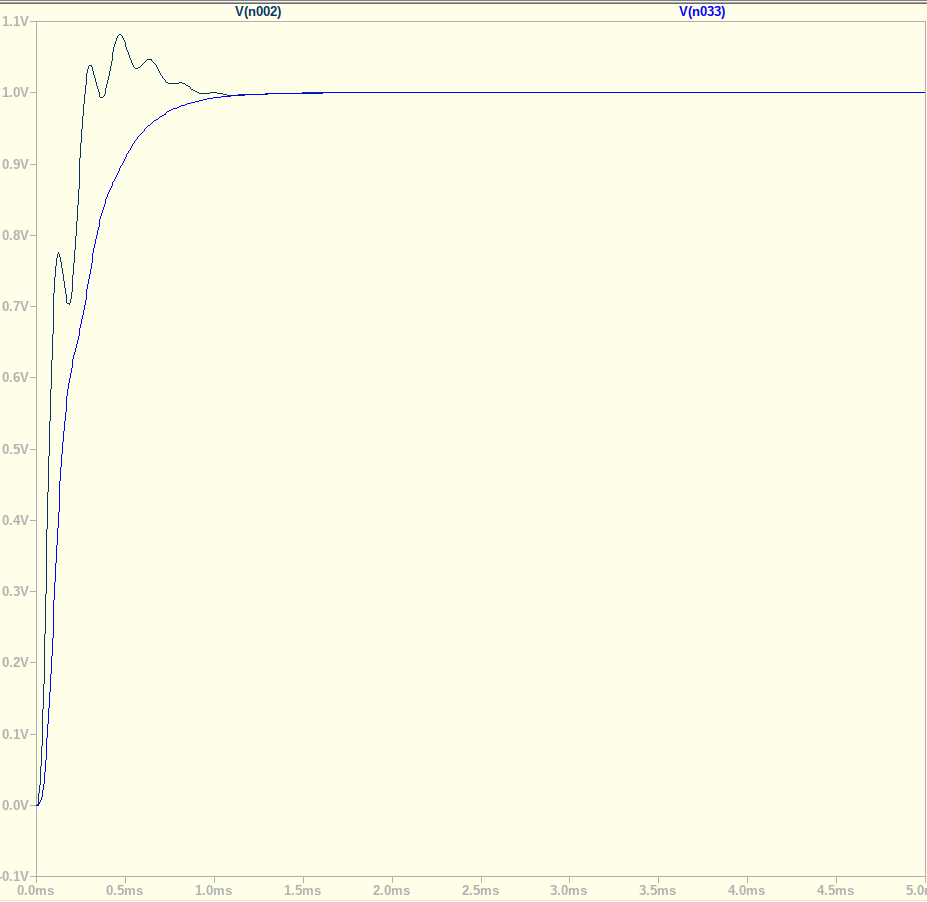
\includegraphics[width=0.7\linewidth]{src/PY_2/Spice_PID.png}
    \caption{Comparación planta sin control y con control}
    \label{fig:placeholder}
\end{figure}

\section{Resultados}

\subsection{Comparación de las Respuestas Simuladas}

La Figura \ref{fig:step} compara la respuesta al escalón de la planta en lazo abierto, el lazo cerrado con la sintonía de Ziegler-Nichols y el lazo cerrado con el ajuste fino. La Tabla \ref{tab:stepinfo} resume las métricas obtenidas con \texttt{stepinfo}.


\begin{figure}[!h]
    \centering
    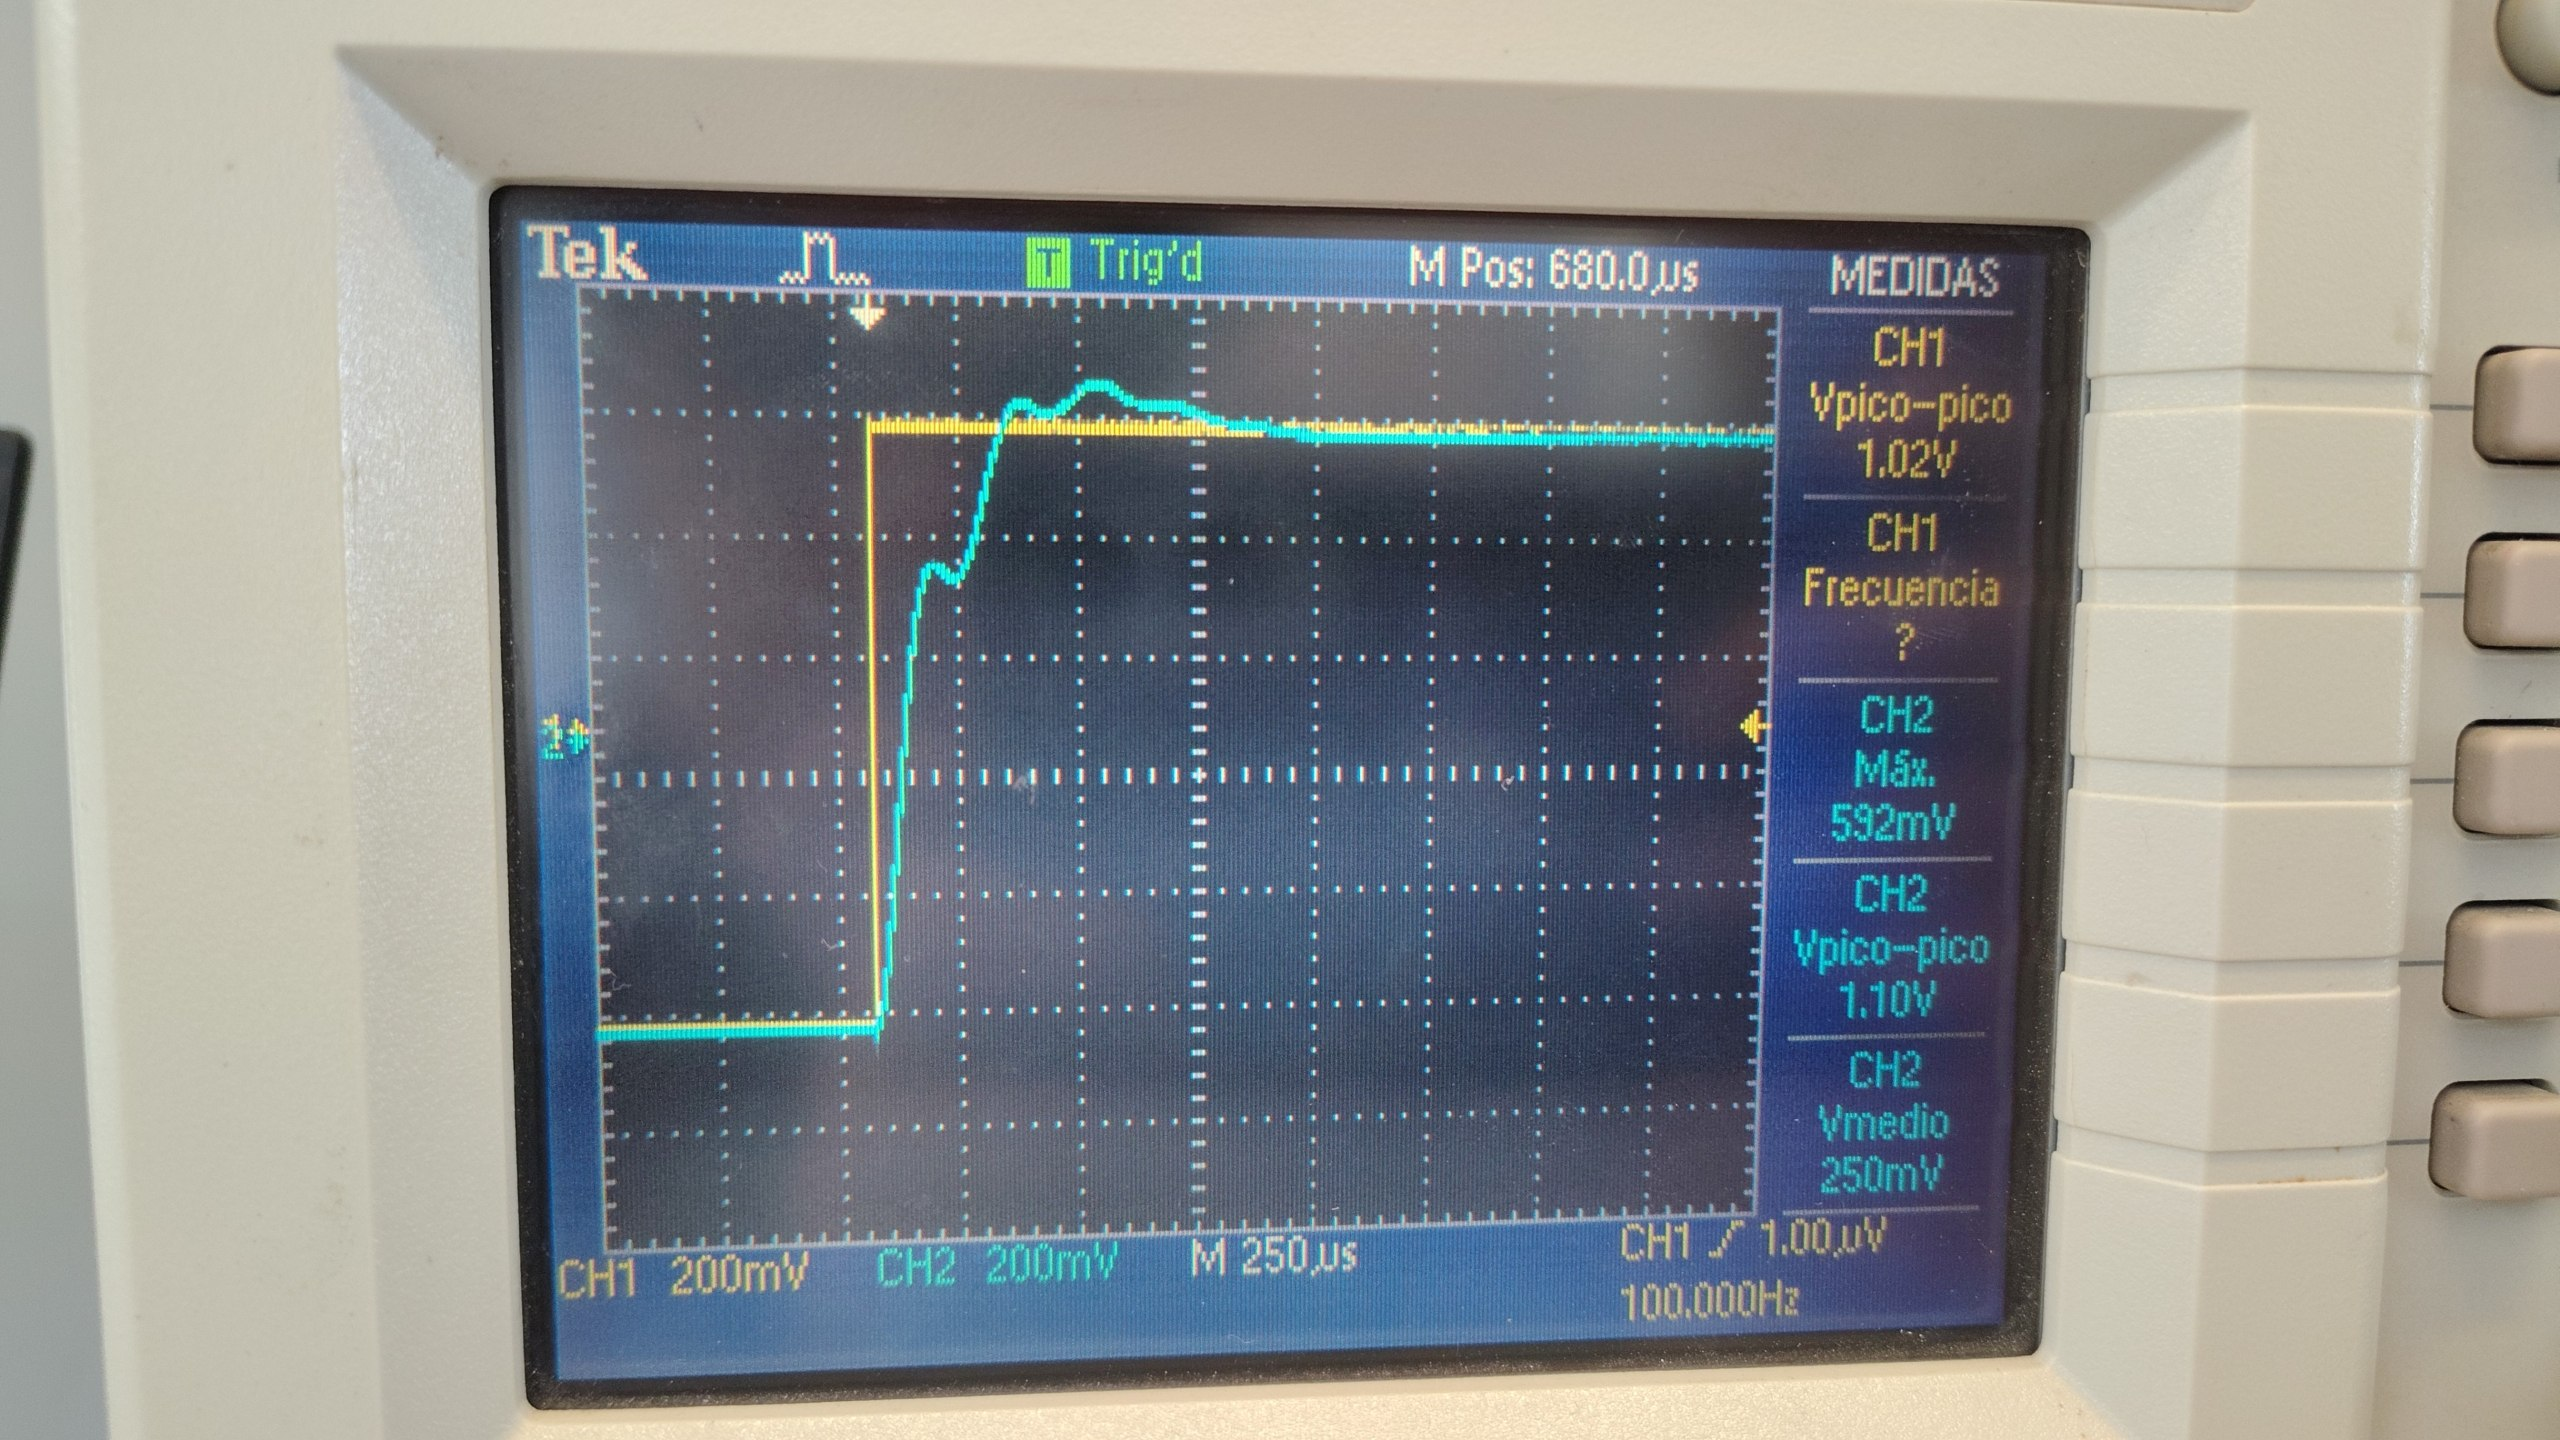
\includegraphics[width=0.8\linewidth]{src/PY_2/Step_Comparacion.png}
    \caption{Respuesta al escalón unitario}
    \label{fig:step}
\end{figure}
\begin{figure}[!h]
    \centering
    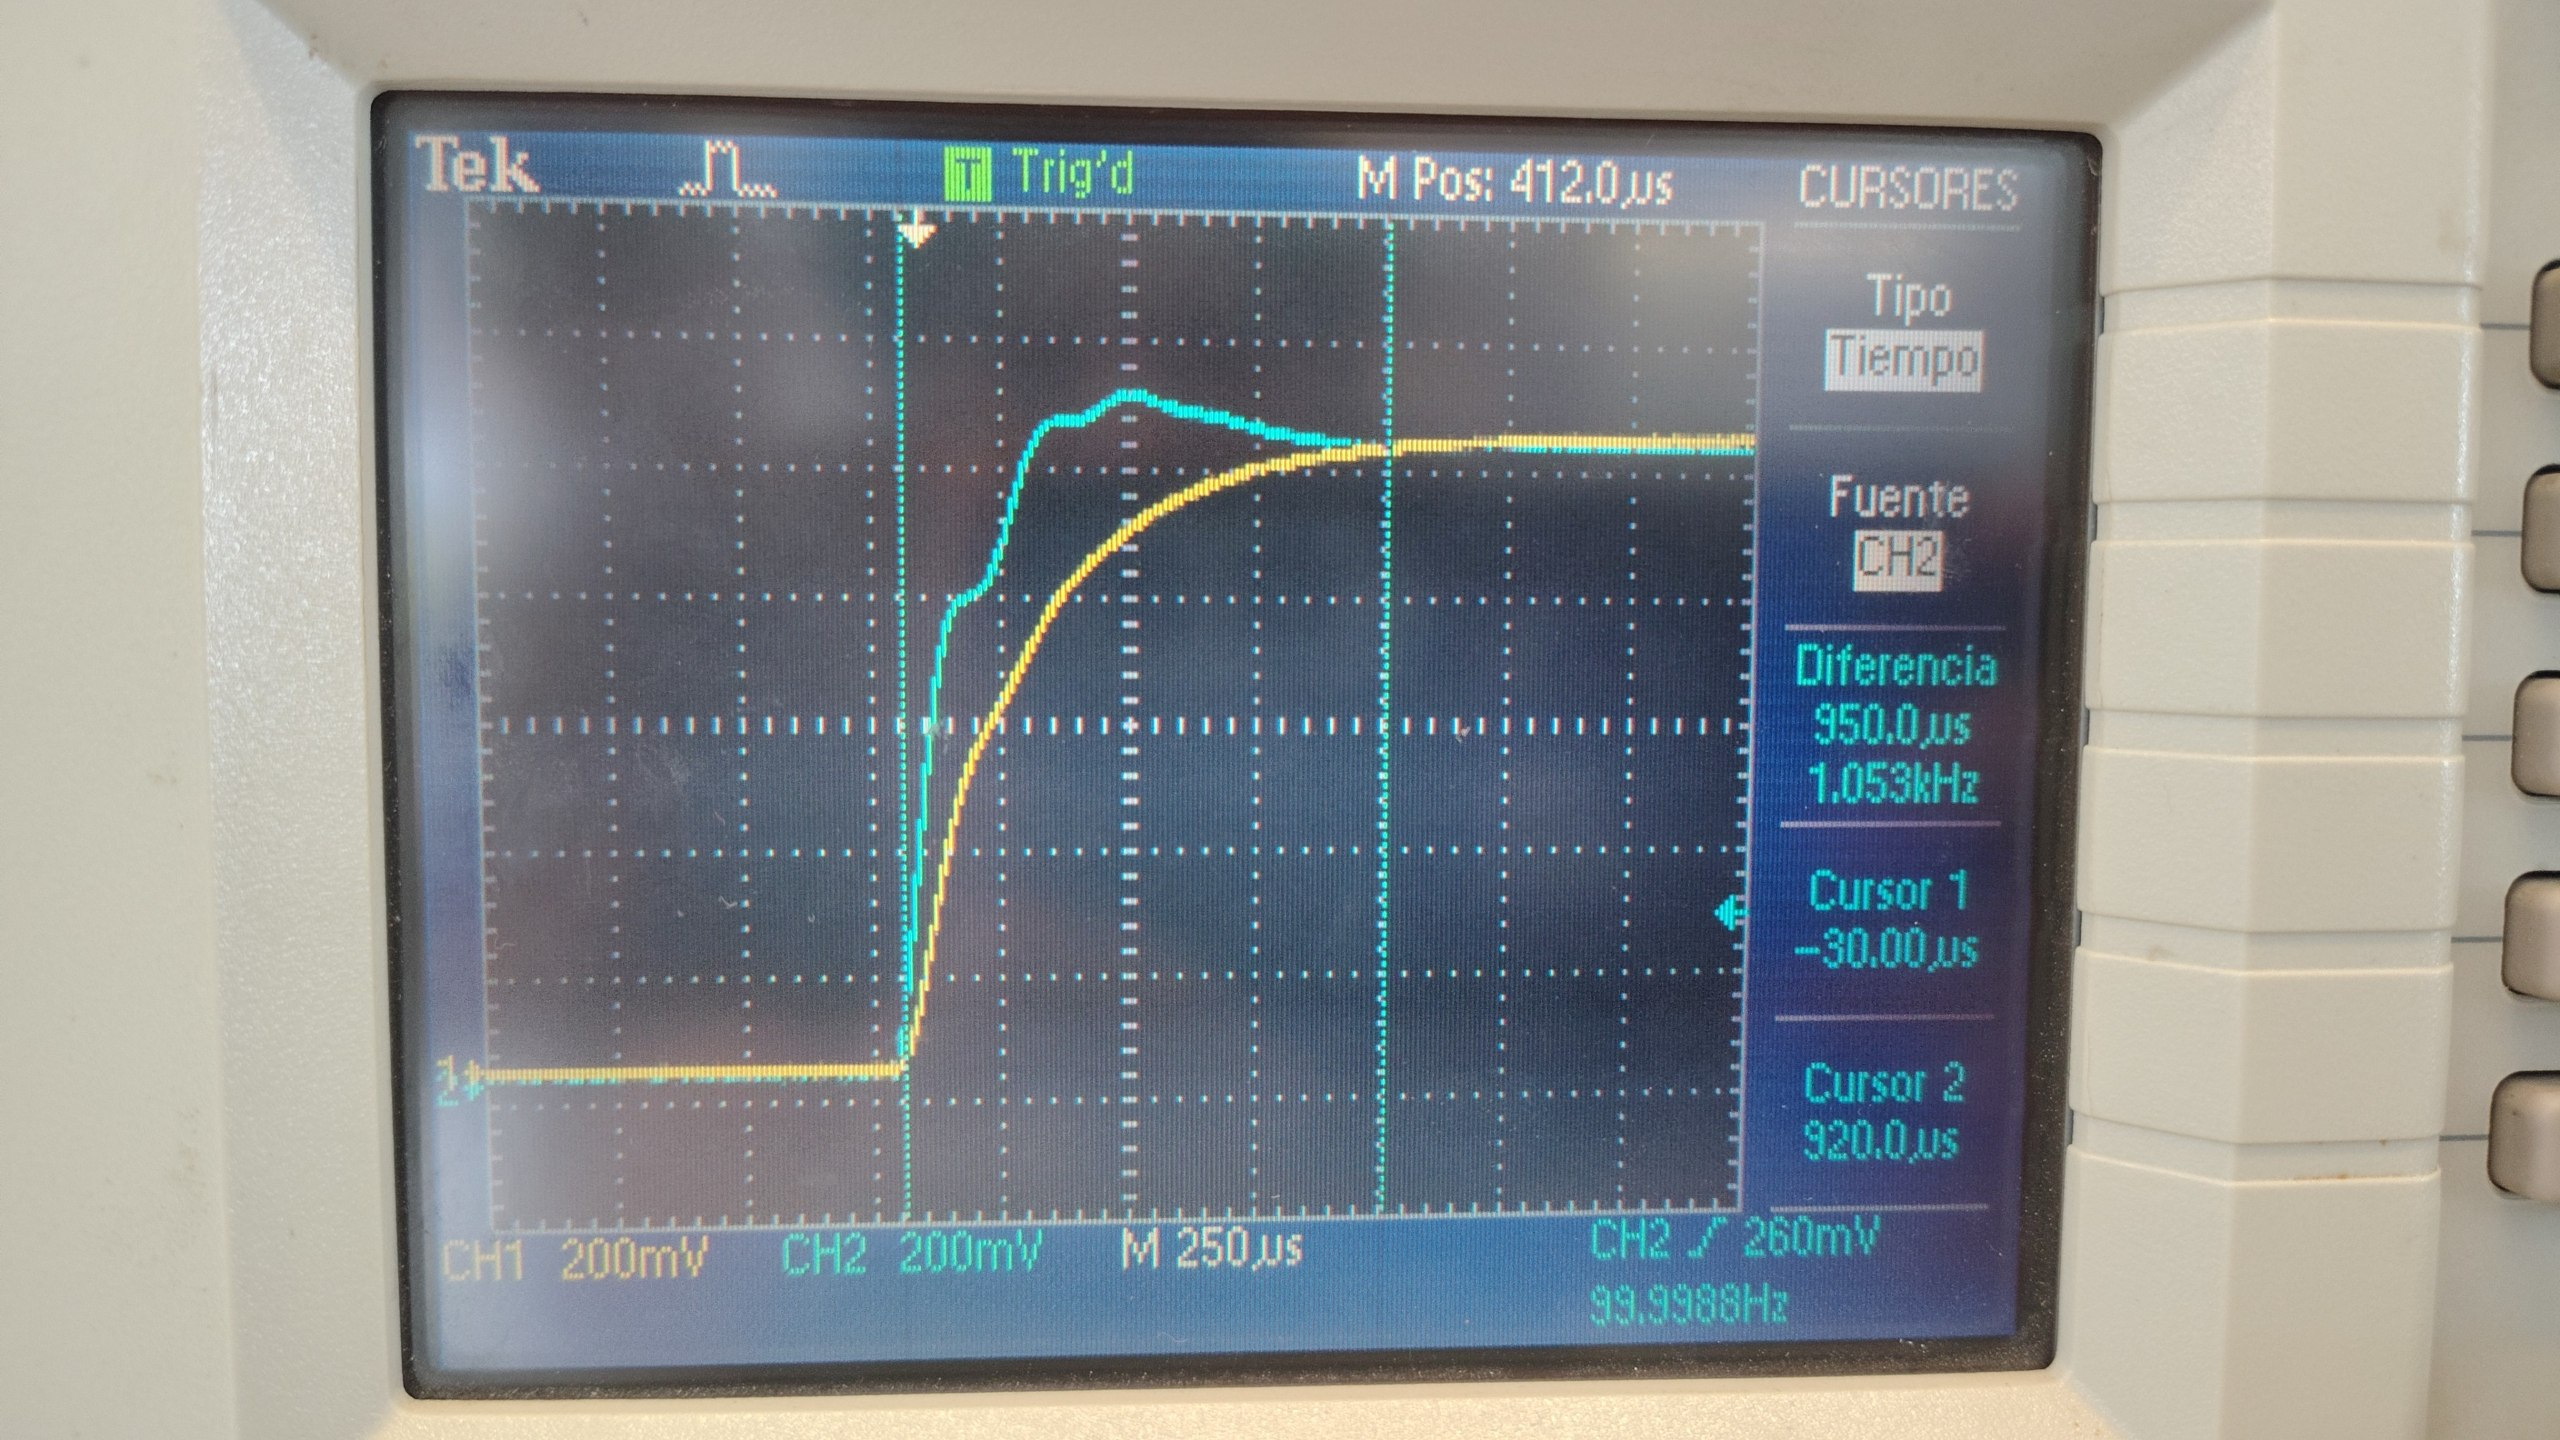
\includegraphics[width=0.8\linewidth]{src/PY_2/LC.png}
    \caption{Comparación planta sin control y con control}
    \label{fig:placeholder}
\end{figure}

\begin{table}[h]
\centering
\caption{Métricas de la respuesta al escalón (criterio de asentamiento del $2\,\%$).}
\label{tab:stepinfo}
\begin{tabular}{lcccc}
\hline
\textbf{Métrica} & \textbf{Lazo abierto} & \textbf{PID Z-N} & \textbf{PID ajustado} & \textbf{PID circuito}$^{*}$ \\
\hline
Tiempo de subida $t_r$ & $422\,\mu\text{s}$ & $71\,\mu\text{s}$ & $213\,\mu\text{s}$ & $212\,\mu\text{s}$ \\
Tiempo pico $t_p$ & -- & $304\,\mu\text{s}$ & $462\,\mu\text{s}$ & $463\,\mu\text{s}$ \\
Sobrepaso $M_p$ & $0\,\%$ & $18.2\,\%$ & $7.6\,\%$ & $8.1\,\%$ \\
Tiempo de asentamiento $t_s$ & $790\,\mu\text{s}$ & $615\,\mu\text{s}$ & $714\,\mu\text{s}$ & $708\,\mu\text{s}$ \\
Error en estado estable $e_{ss}$ & $0$ & $0$ & $0$ & $0$ \\
\hline
\end{tabular}

\vspace{2pt}
{\footnotesize $^{*}$Valores reales de componentes, incluyendo el filtro derivativo ($\tau_f=2.4\,\mu\text{s}$).}
\end{table}

La sintonía de Ziegler-Nichols reduce el tiempo de asentamiento a $615\,\mu\text{s}$, pero su sobrepaso de $18.2\,\%$ no cumple la especificación. El PID con ajuste fino cumple las tres especificaciones: $M_p=7.6\,\%\leq15\,\%$, $e_{ss}=0$ gracias a la acción integral y $t_s=714\,\mu\text{s}<790\,\mu\text{s}$. Además, reduce el tiempo de subida casi a la mitad respecto al lazo abierto ($213$ contra $422\,\mu\text{s}$). Con los valores reales de componentes, el filtro derivativo y la diferencia en $R_{44}$ apenas modifican la respuesta ($M_p=8.1\,\%$, $t_s=708\,\mu\text{s}$).

Cabe señalar que la mejora en el tiempo de asentamiento es moderada ($\approx10\,\%$), ya que la planta de tercer orden no presenta sobrepaso en lazo abierto, y el PID cambia una respuesta lenta sin sobrepaso por una más rápida con un sobrepaso pequeño. La principal ganancia del controlador está en la velocidad de respuesta ($t_r$) y en la robustez del error en estado estable nulo ante variaciones de la planta.

\begin{comment}
    
\subsection{Mediciones Experimentales}

\begin{table}[h]
\centering
\caption{Comparación entre la simulación y la medición experimental.}
\label{tab:medicion}
\begin{tabular}{lcccc}
\hline
\textbf{Métrica} & \textbf{LA simulado} & \textbf{LA medido} & \textbf{LC simulado} & \textbf{LC medido} \\
\hline
$M_p$ & $0\,\%$ & \textcolor{red}{[PENDIENTE]} & $8.1\,\%$ & \textcolor{red}{[PENDIENTE]} \\
$t_s$ ($2\,\%$) & $790\,\mu\text{s}$ & \textcolor{red}{[PENDIENTE]} & $708\,\mu\text{s}$ & \textcolor{red}{[PENDIENTE]} \\
$e_{ss}$ & $0$ & \textcolor{red}{[PENDIENTE]} & $0$ & \textcolor{red}{[PENDIENTE]} \\
$K_{cr}$ & $3.49$ & \textcolor{red}{[PENDIENTE]} & -- & -- \\
$P_{cr}$ & $191.3\,\mu\text{s}$ & \textcolor{red}{[PENDIENTE]} & -- & -- \\
\hline
\end{tabular}
\end{table}
\end{comment}

\section{Análisis y Discusión}

Las diferencias esperadas entre la simulación y la medición se deben a varios factores:

\begin{itemize}
    \item \textbf{Resistencia DC del inductor y resistencia de salida del amplificador:} ambas se suman a los $158\,\Omega$ de la resistencia serie, por lo que incrementan $\zeta$. Por ejemplo, una DCR de $20\,\Omega$ elevaría $\zeta$ de $0.25$ a $0.28$, lo que modifica $K_{cr}$ y $P_{cr}$.
    \item \textbf{Tolerancias de los componentes:} un error de $\pm10\,\%$ en $L$ o $C$ desplaza $\omega_n$ cerca de un $\pm5\,\%$. Las tolerancias de $R_{49}$ y $C_{14}$ cambian el polo dominante de la etapa RC, que es el que más influye en el tiempo de asentamiento.
    \item \textbf{Producto ganancia-ancho de banda (GBW):} el TL082 tiene un GBW de $3\,\text{MHz}$. A la frecuencia de oscilación ($5.23\,\text{kHz}$) las ramas P e I operan sin problema, pero el derivador tiene ganancia alta en frecuencia, por lo que su respuesta real se aparta del modelo ideal por encima de unos cientos de kHz y añade un desfase adicional al lazo.
    \item \textbf{Saturación y slew rate:} el pico derivativo ante el escalón satura la rama D durante algunos microsegundos. Además, el slew rate del TL082 ($13\,\text{V}/\mu\text{s}$) limita la rapidez de ese pico.
    \item \textbf{Limitaciones del método de Ziegler-Nichols:} es una regla empírica que busca una razón de decaimiento de aproximadamente $1/4$, por lo que suele producir sobrepasos altos ($18.2\,\%$ en este caso). Además, requiere llevar el sistema al límite de estabilidad, lo que en un sistema real implica el riesgo de saturar los amplificadores durante la prueba. Por ello, la sintonía obtenida se toma solo como punto de partida para el ajuste fino.
\end{itemize}

\section{Conclusiones}

Se diseñó un controlador PID analógico en forma paralela para una planta RLC de tercer orden con $\omega_n=31.62\,\text{krad/s}$ y $\zeta=0.25$. La etapa RC adicional permitió que la planta alcanzara el límite de estabilidad con una ganancia proporcional finita ($K_{cr}=3.49$, $P_{cr}=191.3\,\mu\text{s}$), lo que hizo posible aplicar el método de oscilaciones sostenidas de Ziegler-Nichols.

La sintonía de Ziegler-Nichols ($K_p=2.09$, $T_i=95.6\,\mu\text{s}$, $T_d=23.9\,\mu\text{s}$) produjo una respuesta rápida pero con un sobrepaso de $18.2\,\%$, que no cumple la especificación. El ajuste fino en MATLAB, que redujo $K_p$ y $K_i$ y aumentó $K_d$, llevó a $K_p=1.5$, $K_i=1.2\times10^{4}\,\text{s}^{-1}$ y $K_d=6.7\times10^{-5}\,\text{s}$, con lo que se cumplen las tres especificaciones: $M_p=7.6\,\%$, $e_{ss}=0$ y $t_s=714\,\mu\text{s}$, menor que los $790\,\mu\text{s}$ de lazo abierto, con márgenes de estabilidad amplios ($28.5\,\text{dB}$ y $81.6^\circ$). La simulación con los valores reales de componentes y con saturación de $\pm12\,\text{V}$ confirmó que el diseño mantiene su desempeño ($M_p=8.6\,\%$, $t_s=717\,\mu\text{s}$).

Como áreas de mejora, se identificó que el polo de la etapa RC ($5\,000\,\text{rad/s}$) domina la dinámica de la planta y limita la mejora alcanzable en el tiempo de asentamiento; reducir $\tau$ acercaría el comportamiento al del RLC y dejaría más margen al controlador.


\begin{thebibliography}{9}
\bibitem{ogata} K. Ogata, \textit{Ingeniería de Control Moderna}, 5.ª ed. Madrid: Pearson, 2010.
\bibitem{zn} J. G. Ziegler y N. B. Nichols, ``Optimum settings for automatic controllers,'' \textit{Transactions of the ASME}, vol. 64, pp. 759--768, 1942.
\bibitem{astrom} K. J. Åström y T. Hägglund, \textit{PID Controllers: Theory, Design, and Tuning}, 2.ª ed. Research Triangle Park, NC: ISA, 1995.
\bibitem{tl082} Texas Instruments, \textit{TL08xx JFET-Input Operational Amplifiers}, hoja de datos.
\end{thebibliography}

\begin{figure}[!h]
    \centering
    
\includegraphics[width=0.9\linewidth]{src/PY_2/QR.png}
    \label{fig:placeholder}
\end{figure}
\end{document}